\documentclass[a4paper, 12pt, final, garamond]{book}
\usepackage{cours-preambule}

\raggedbottom

\makeatletter
\renewcommand{\@chapapp}{M\'ecanique -- chapitre}
\makeatother

\toggletrue{student}
% \HideSolutionstrue
\toggletrue{corrige}
\renewcommand{\mycol}{black}
% \renewcommand{\mycol}{gray}

\begin{document}
\setcounter{chapter}{4}

\chapter{\cswitch{Correction du TD d'application}{TD application~: mouvement de
	  particules charg\'ees}}

\resetQ
\section{Mouvements simples de particules chargées}

\enonce{%
	On considère une particule ponctuelle, de charge $q$ et de masse $m$, de vitesse
	initiale $\vfo$ à l'entrée d'une zone où règnent un champ électrique $\Ef$ ou un
	champ magnétique $\Bf$. On suppose ces champs uniformes et indépendants du
	temps, et on néglige toute autre force que celles provoquées par ces champs.
	\smallbreak
	On suppose dans un premier temps que la particule décrit une droite et possède
	une accélération constante $a$.
}

\QR{%
	Déterminer la direction et la norme du ou des champs qui provoquent
	cette trajectoire.
}{%
	On étudie la particule M de masse $m$ et de charge $q$ assimilée à
	un point matériel dans le référentiel du laboratoire supposé galiléen.
	Cette particule est soumise à la force de \textsc{Lorentz}
	\[
		\Ff = q(\Ef+\vf\wedge \Bf)
	\]
	La trajectoire est rectiligne et uniformément accélérée, soit
	\[
		\frac{\dd \vf}{\dd t}
		= \af
		= \vcte
		\quad \Ra \quad
		\vf = \af t + \vfo
	\]
	La norme de $\vf$ varie, donc l'énergie cinétique aussi. Or,
	\textbf{seule la force électrique travaille}\footnote{La force de
		\textsc{Lorentz} magnétique $q (\vf\wedge\Bf)$ est perpendiculaire à
		$\vf$ donc à la trajectoire}, le champ est un donc champ électrique. De
	plus, pour que la trajectoire soit rectiligne, il faut, d'après
	l'expression de $\vf(t)$, que $\af$ soit colinéaire à $\vfo$. Or,
	\[
		\af = \frac{q}{m}\Ef
	\]
	donc \textbf{$\Ef$ est colinéaire à $\vfo$}.
}

\QR{%
	Déterminer la position $\OM$ du point en fonction du temps. On
	notera $\OM_0$ la position initiale.
}{%
	On note O l'origine du repère. On intègre l'expression de la vitesse
	pour avoir la position $\OM$ de la particule~:
	\[
		\boxed{\OM = \frac{q}{2m} t^2 \, \Ef + t \vfo + \OM_0}
	\]
}

\enonce{%
	La particule décrit maintenant une trajectoire circulaire de rayon $R_0$, dans
	un plan $x\Or y$.
}

\QR{%
	Déterminer la direction du ou des champs qui provoquent cette
	trajectoire.
}{%
	La trajectoire circulaire est celle d'une charge dans un champ
	magnétique perpendiculaire à la vitesse initiale. On en déduit que
	\textbf{$\Bf$ est suivant $\Or z$ et que $\vfo$ est dans le plan $x\Or
			y$}.
}

\QR{%
	Déterminer l'équation de la trajectoire et la relation entre la norme
	du champ, $v_0$ et $R_0$. On suggère d'utiliser les coordonnées
	polaires.
}{%
	La trajectoire étant circulaire, la vitesse en coordonnées polaires a
	pour expression $\vf = R_0 \tp \ut$ et
	l'accélération se réduit à
	\[
		\af = -R_0 \tp^2 \ur + R_0 \tpp \ut
	\]

	Le principe fondamental de la dynamique, appliqué à la charge $q$ dans
	le référentiel d'étude que l'on supposera galiléen, s'écrit~:
	\[
		m \af = q \vf \wedge \Bf
	\]

	Or, $\Bf = B \uz$. Par conséquent,

	\begin{align*}
		q \vf \wedge \Bf        & = qR_0\tp\ut\wedge B\uz
		\\
		                        & = qBR_0\tp(\underbracket[1pt]{\ut\wedge\uz}_{=\ur})
		\\\Lra
		\Aboxed{q\vf \wedge \Bf & = qBR_0\tp\ur}
	\end{align*}
	En projetant le PFD sur la base polaire $(\ur, \ut)$, il vient~:
	\begin{empheq}[left=\empheqlbrace]{align*}
		-mR_0 \tp^2 & = qR_0 \tp B\\
		R_0 \tpp    & = 0
	\end{empheq}
	On obtient alors
	\[
		\boxed{\tp = -\frac{qB}{m} = \cte
			\quad\Ra\quad
			\tt(t) = -\frac{qB}{m}t + \tt_0}
	\]

	Si la charge est positive, elle tourne dans le sens anti-trigonométrique
	(horaire) par rapport à $\Or z$. Puisque $\tp$ est constante, le
	mouvement et circulaire uniforme et $v_0 = R_0 \abs{\tp}$ (c'est une
	norme donc nécessairement positive~!) d'où
	\[
		\boxed{R_0 = \frac{mv_0}{qB}}
	\]
}

\resetQ
\section{Filtre de vitesse}

\enonce{%
	\noindent
	\begin{minipage}[c]{0.50\linewidth}
		Un ion de masse $m$ et de charge $q$ pénètre dans un filtre par la fente $F_1$
		avec un vecteur vitesse $\vf = v_0\ux$. Il y règne un champ électrique $\Ef =
			E\uy$ et un champ magnétique $\Bf$ = $B\uz$, uniformes et stationnaires.
	\end{minipage}
	\hfill
	\begin{minipage}[c]{0.50\linewidth}
		\begin{center}
			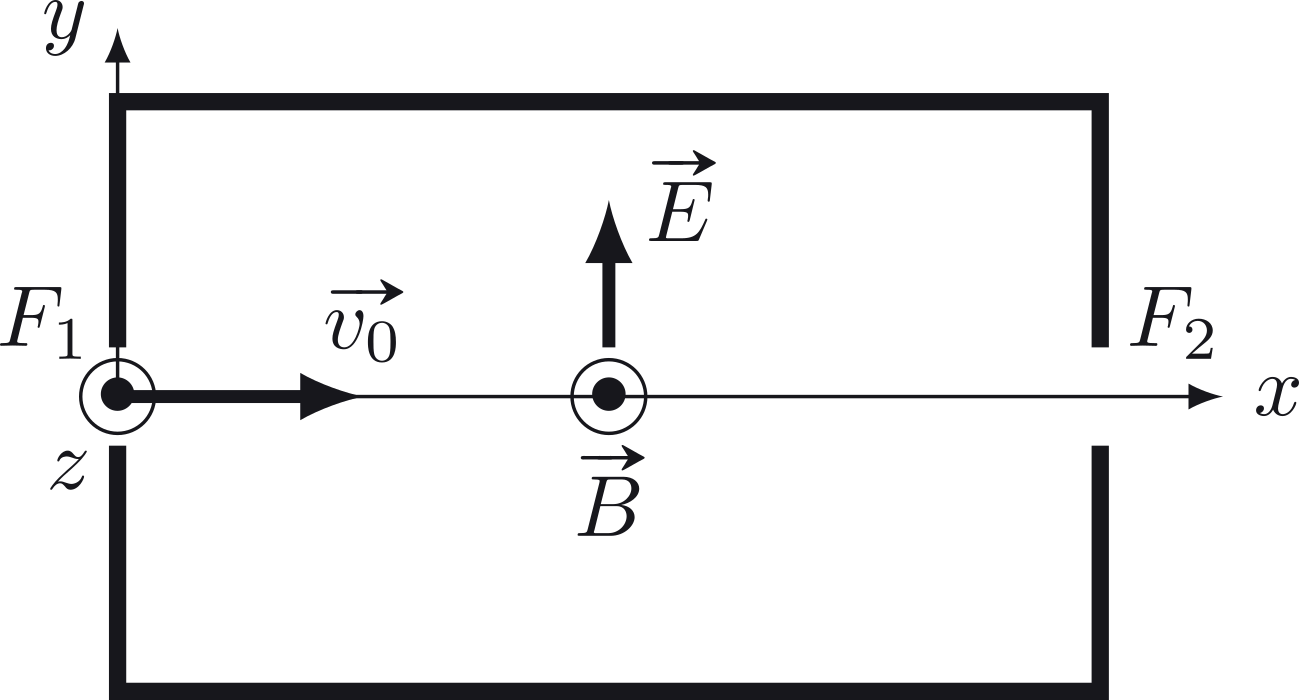
\includegraphics[width=5cm]{filtre_vitesse-plain}
			\captionof{figure}{Schéma du filtre de vitesse.}
			\label{fig:fdv}
		\end{center}
	\end{minipage}
}

\QR{%
	Écrire la force de \textsc{Lorentz} alors ressentie par l'ion.
}{%
	Dans le référentiel du laboratoire, le système \{ion\} repéré par son
	point matériel M de masse $m$ et de charge $q$ dans un repère cartésien
	$(F_1,\ux,\uy,\uz)$ est soumis à la force de \textsc{Lorentz}, telle que
	\begin{align*}
		\Ff         & = q\left(\Ef + \vf\wedge\Bf\right)
		\\
		            & = qE\uy + qBv_0\,(\underbracket[1pt]{\ux\wedge\uz}_{=-\uy})
		\\\Lra
		\Aboxed{\Ff & = q(E-Bv_0)\,\uy}
	\end{align*}
}
\QR{%
	À quelle condition l'ion peut-il avoir une trajectoire rectiligne
	l'amenant à passer à travers la fente $F_2$~?
}{%
	Pour avoir une trajectoire rectiligne sur $\ux$, il faut que la somme
	des forces s'appliquant sur l'ion soit nulle. Ainsi, en négligeant le poids
	devant la force de \textsc{Lorentz}, il faut \textbf{que la force de
		\textsc{Lorentz} soit nulle}.
}
\QR{%
	Exprimer en fonction de $E$ et $B$ la vitesse $v_0$ lui permettant
	d'atteindre la fente $F_2$. Justifier le nom du dispositif.
}{%
	La condition précédente avec l'équation de la première question amène
	à
	\[E-v_0B = 0 \Lra \boxed{v_0 = \frac{E}{B}}\]
	Ainsi, si le vecteur vitesse de la particule n'est pas égal à $v_0\ux$,
	alors elle sera déviée et ne passera pas par la fente $F_2$~: on filtre
	effectivement les vitesses.
}

\resetQ
\section{Déviation d'un électron}

\enonce{%
	\noindent
	\begin{minipage}[c]{0.50\linewidth}
		Un électron pénètre en $A$ avec une vitesse initiale $\vfo$ dans la zone
		grisée où règne un champ magnétique $\Bf$ uniforme et stationnaire. On
		suppose que la zone où règne le champ magnétique est très grand de telle
		sorte que la particule ne peut que ressortir par les côtés AC ou AD.
	\end{minipage}
	\hfill
	\begin{minipage}[c]{0.50\linewidth}
		~
		\begin{center}
			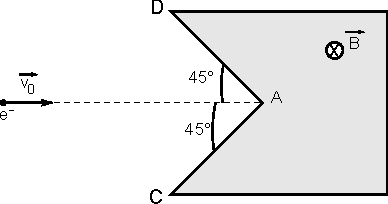
\includegraphics[width=5cm]{miroir_mag-plain}
			\captionof{figure}{Schéma de la situation.}
			\label{fig:mirmag}
		\end{center}
	\end{minipage}
}

\QR{%
	Quelle est la trajectoire de la particule dans la zone grisée~? On
	précisera les caractéristiques de cette trajectoire.
}{%
	La particule arrive dans un champ magnétique uniforme et stationnaire
	${\Bf=\vcte}$ avec une vitesse $\vfo=v_0\ex$ orthogonale à $\Bf$. La
	trajectoire est donc un cercle de rayon $R=mv_0/(qB_0)$, avec
	$B_0=\norm{\Bf}$. La force en A est dirigée vers le bas, on en déduit la
	position du centre C$_1$ de la trajectoire.

	\begin{center}
		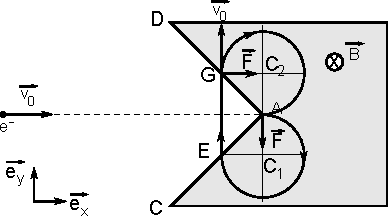
\includegraphics[width=.5\linewidth]{miroir_mag-corr}
		\captionof{figure}{Trajectoire dans la zone.}
		\label{fig:miroir_mag_corr}
	\end{center}
}
\QR{%
	Par quelle face ressort la particule~? Quelle est la direction de la
	vitesse~?
}{%
	La particule ressort par la face AC en E, avec une vitesse selon
	$\ey$ car le triangle AC$_1$E est isocèle et rectangle en C$_1$.
}

\QR{%
	Que se passe-t-il ensuite~? Quel nom donneriez-vous à ce dispositif~?
}{%
	En dehors de la zone grisée, la particule est isolée, donc elle est
	animée d'un mouvement rectiligne uniforme ($\vf=v_0\ey=\vcte$) dans le
	référentiel du laboratoire supposé galiléen. \bigbreak

	La particule entre à nouveau dans le zone où règne le champ magnétique
	par la face AD, avec une vitesse $\vf=v_0\ey$. La trajectoire est
	alors circulaire de même rayon $R$ (car la vitesse est la même en
	norme). On représente la force magnétique en G, et on en déduit le
	position C$_2$ du centre de la trajectoire. La particule arrive en A
	avec la vitesse $\vf=-v_0\ex$ et sort de la zone grisée. \bigbreak

	Au final, la particule a subi une déviation de $\pi$, comme si elle
	avait été réfléchie par un miroir. On pourrait donc appeler ce
	dispositif un \textbf{miroir magnétique}.

	\begin{tcb}(rema)<lft>'l'{Remarque}
		Vérifiez que l'effet miroir est maintenu si la particule incidente
		n'arrive plus en A. On constate en revanche que la particule
		n'emprunte plus le même chemin qu'à l'aller.
	\end{tcb}
}

\resetQ
\section{Imprimante jet d'encre}

\enonce{%
	Dans un dispositif d'impression industriel, les gouttelettes d'encre sont
	chargées puis déviées de manière contrôlée par un déflecteur électrostatique
	avant d'atteindre le support d'impression.

	\noindent
	\begin{minipage}[t]{0.45\linewidth}
		Un gouttelette de volume $V = \SI{10}{pL}$, de charge $q = \SI{3.4e-14}{C}$
		et de vitesse $v_0 = \SI{20}{m.s^{-1}}$ entre en O dans le déflecteur,
		constitué de deux électrodes planes portées aux potentiels électriques $V_1$
		et $V_2$ et générant un champ électrostatique uniforme $\Ef = E\uy$ avec $E
			= \SI{5.0e5}{V.m^{-1}}$. \bigbreak
		La longueur du déflecteur est $L_1 = \SI{5.0}{cm}$. Le support d'impression
		se trouve à la distance $L_2 = \SI{20}{cm}$ de la sortie du déflecteur.
		L'encre est essentiellement constituée d'eau, de masse volumique $\rho =
			\SI{1.0e3}{kg.m^{-3}}$.
	\end{minipage}
	\hfill
	\begin{minipage}[t]{0.45\linewidth}
		~\vspace{-12pt}
		\begin{center}
			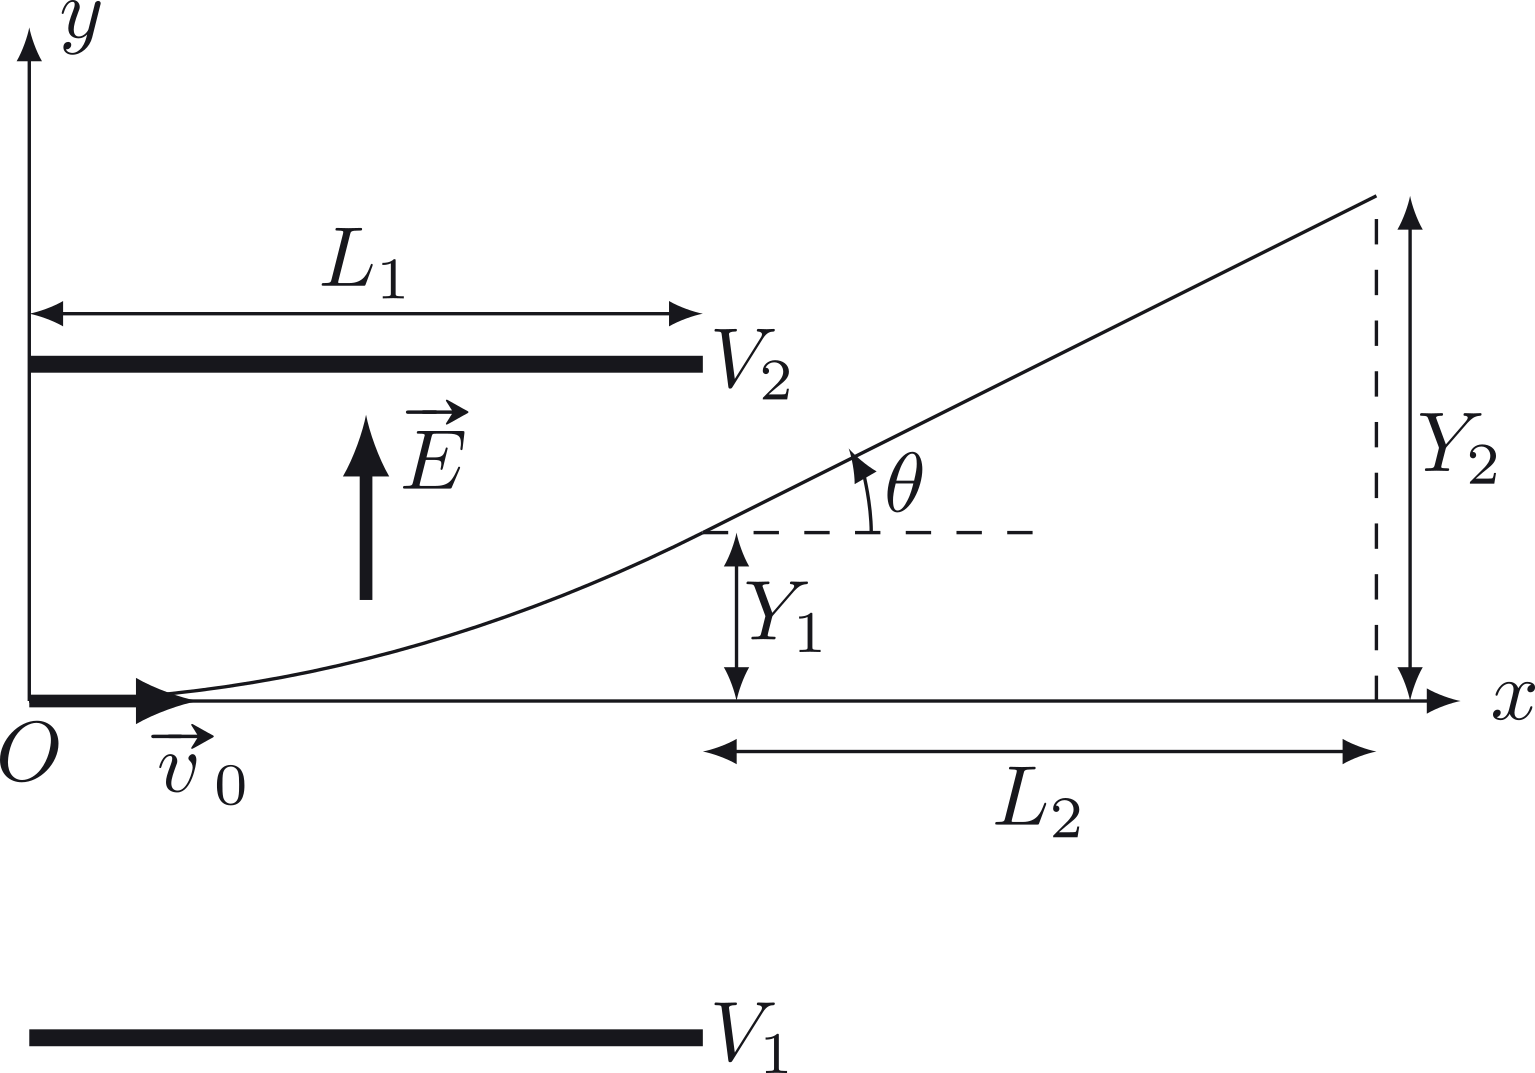
\includegraphics[width=\linewidth]{deflecteur_plain}
			\captionof{figure}{Schéma du déflecteur.}
			\label{fig:deflec}
		\end{center}
	\end{minipage}
}

\QR{%
	Quel est le signe de la tension $V_1 - V_2$ pour que la gouttelette
	d'encre soit effectivement déviée dans le sens des $y$ croissants~?
}{%
	La gouttelette est chargée positivement, et subit la force électrique
	$\Ff_e = q\Ef$. Pour aller dans le sens des $y$ croissants, il faut que
	$\Ef$ soit selon $\uy$, comme indiqué dans l'énoncé. Or, $\Ef = -\gd V$,
	donc $\Ef$ va des \textbf{hauts potentiels} vers les \textbf{bas
		potentiels}~; il faut donc $V_1 > V_2$, soit
	\[\boxed{V_1 - V_2 > 0}\]
}

\QR{%
	Calculer la masse $m$ de la gouttelette et montrer que l'on peut
	négliger son poids devant la force électrique de \textsc{Lorentz}.
}{%
	La gouttelette a un volume $V$ et une masse volumique $\rho$. On en
	déduit
	\begin{gather*}
		\boxed{m = \rho V}
		\qavec
		\left\{
		\begin{array}{rcl}
			\rho & = & \SI{1.0e3}{kg.m^{-3}}             \\
			V    & = & \SI{10}{pL} = \SI{10e-12}{(dm)^3} \\
			     & = & \SI{1.0e-11}{(10^{-1}m)^3}        \\
			     & = & \SI{1.0e-14}{m^3}
		\end{array}
		\right.\\\AN
		\boxed{m = \SI{1.0e-11}{kg}}
	\end{gather*}
	Ainsi, on trouve
	\[
		\norm{\Ff_e} = qE \approx \SI{1.7e-8}{N}
		\qet
		\norm{\Pf} = mg \approx \SI{1.0e-10}{N}
		\qsoit
		\boxed{\norm{\Ff_e} \approx 200\times\norm{\Pf}}
	\]
	On peut donc négliger le poids devant la force de \textsc{Lorentz}.
}
\QR{%
Appliquer la deuxième loi de \textsc{Newton} à la gouttelette entre
les électrodes et déterminer l'équation de sa trajectoire. En déduire le
déplacement $Y_1$ en sortie du déflecteur.
}{%
On applique le PFD à la gouttelette dans le référentiel de la salle
d'impression, supposé galiléen, avec un repère cartésien tel qu'indiqué
sur le schéma~:
\begin{gather*}
	m\af = q\Ef
	\Ra
	\left\{
	\begin{aligned}
		m\xpp & = 0  \\
		m\ypp & = 0  \\
		m\zpp & = qE
	\end{aligned}
	\right.
	\Ra
	\left\{
	\begin{aligned}
		\xp & = v_0           \\
		\yp & = \frac{qE}{m}t
	\end{aligned}
	\right.
	\Ra
	\left\{
	\begin{aligned}
		x(t) & = v_0t             \\
		y(t) & = \frac{qE}{2m}t^2
	\end{aligned}
	\right.
\end{gather*}
en intégrant une première fois avec $\xp(0) = v_0$ et $\yp(0) = 0$, en
ignorant le mouvement en $z$, puis en intégrant une seconde fois, avec
$x(0) = 0 = y(0)$.  On trouve alors l'équation de la trajectoire~:
\[\boxed{y(x) = \frac{qE}{2mv_0{}^2}x^2}\]
qui est l'équation d'une parabole. Ainsi, on trouve $Y_1 = y(L_1)$~:
\[\boxed{Y_1 = \SI{5.3e-3}{m} = \SI{5.3}{mm}}\]


}
\QR{%
	Caractériser la trajectoire de la gouttelette après sa sortie du
	déflecteur, en négligeant son poids.
}{%
	Après être sortie du déflecteur, la gouttelette n'est soumise à aucune
	action sauf son poids, que l'on ignore sur la durée du trajet restant
	($v_0 = \SI{20}{m.s^{-1}}$)~: sa trajectoire est donc rectiligne et
	uniforme.
}

\QR{%
Exprimer puis calculer la déflexion angulaire $\tt$. En déduire le
déplacement $Y_2$.
}{%
On trouve l'angle de sortie en prenant
\[\tan\tt = \dv{y}{x} = \frac{\yp(L_1)}{\xp(L_1)} =
	\frac{qEL_1}{mv_0{}^2} = 2\frac{Y_1}{L_1}\]
L'angle trouvé étant petit ($\tt \approx \SI{0.21}{rad}$), $\tan\tt
	\approx \tt \approx \sin\tt$. Or, on a
\begin{gather*}
	Y_2 = Y_1 + L_2\sin\tt
	\\\Ra
	\boxed{Y_2 = Y_1\left(1+2\frac{L_2}{L_1}\right)}
	\qavec
	\left\{
	\begin{array}{rcl}
		Y_1 & = & \SI{5.3e-1}{cm} \\
		L_1 & = & \SI{5.0}{cm}    \\
		L_2 & = & \SI{20}{cm}
	\end{array}
	\right.\\\AN
	\boxed{Y_2 = \SI{4.8}{cm}}
\end{gather*}
}

\end{document}
